%-----------------------------------------------------------------------------------------------------------------------------------------------%
%	The MIT License (MIT)
%
%   Copyright (c) 2021 Mike Lubibets
%	Copyright (c) 2021 Philip Empl (original template authorship)
%
%	Permission is hereby granted, free of charge, to any person obtaining a copy
%	of this software and associated documentation files (the "Software"), to deal
%	in the Software without restriction, including without limitation the rights
%	to use, copy, modify, merge, publish, distribute, sublicense, and/or sell
%	copies of the Software, and to permit persons to whom the Software is
%	furnished to do so, subject to the following conditions:
%	
%	THE SOFTWARE IS PROVIDED "AS IS", WITHOUT WARRANTY OF ANY KIND, EXPRESS OR
%	IMPLIED, INCLUDING BUT NOT LIMITED TO THE WARRANTIES OF MERCHANTABILITY,
%	FITNESS FOR A PARTICULAR PURPOSE AND NONINFRINGEMENT. IN NO EVENT SHALL THE
%	AUTHORS OR COPYRIGHT HOLDERS BE LIABLE FOR ANY CLAIM, DAMAGES OR OTHER
%	LIABILITY, WHETHER IN AN ACTION OF CONTRACT, TORT OR OTHERWISE, ARISING FROM,
%	OUT OF OR IN CONNECTION WITH THE SOFTWARE OR THE USE OR OTHER DEALINGS IN
%	THE SOFTWARE.
%	
%
%-----------------------------------------------------------------------------------------------------------------------------------------------%


%============================================================================%
%
%	DOCUMENT DEFINITION
%
%============================================================================%

\documentclass[10pt,A4,english]{article}	


%----------------------------------------------------------------------------------------
%	ENCODING
%----------------------------------------------------------------------------------------

% we use utf8 since we want to build from any machine
\usepackage[utf8]{inputenc}		
\usepackage[USenglish]{isodate}
\usepackage{fancyhdr}
\usepackage[numbers]{natbib}

%----------------------------------------------------------------------------------------
%	LOGIC
%----------------------------------------------------------------------------------------

% provides \isempty test
\usepackage{xstring, xifthen}
\usepackage{enumitem}
\usepackage[english]{babel}
\usepackage{blindtext}
\usepackage{pdfpages}
\usepackage{changepage}
%----------------------------------------------------------------------------------------
%	FONT BASICS
%----------------------------------------------------------------------------------------

% some tex-live fonts - choose your own

%\usepackage[defaultsans]{droidsans}
%\usepackage[default]{comfortaa}
%\usepackage{cmbright}
\usepackage[default]{raleway}
%\usepackage{fetamont}
%\usepackage[default]{gillius}
%\usepackage[light,math]{iwona}
%\usepackage[thin]{roboto} 

% set font default
\renewcommand*\familydefault{\sfdefault} 	
\usepackage[T1]{fontenc}

% more font size definitions
\usepackage{moresize}

%----------------------------------------------------------------------------------------
%	FONT AWESOME ICONS
%---------------------------------------------------------------------------------------- 

% include the fontawesome icon set
\usepackage{fontawesome}

% use to vertically center content
% credits to: http://tex.stackexchange.com/questions/7219/how-to-vertically-center-two-images-next-to-each-other
\newcommand{\vcenteredinclude}[1]{\begingroup
\setbox0=\hbox{\includegraphics{#1}}%
\parbox{\wd0}{\box0}\endgroup}
\newcommand{\tab}[1]{\hspace{.2\textwidth}\rlap{#1}}
% use to vertically center content
% credits to: http://tex.stackexchange.com/questions/7219/how-to-vertically-center-two-images-next-to-each-other
\newcommand*{\vcenteredhbox}[1]{\begingroup
\setbox0=\hbox{#1}\parbox{\wd0}{\box0}\endgroup}

% icon shortcut
\newcommand{\icon}[3] { 							
	\makebox(#2, #2){\textcolor{maincol}{\csname fa#1\endcsname}}
}	


% icon with text shortcut
\newcommand{\icontext}[4]{ 						
	\vcenteredhbox{\icon{#1}{#2}{#3}}  \hspace{2pt}  \parbox{0.9\mpwidth}{\textcolor{#4}{#3}}
}

% icon with website url
\newcommand{\iconhref}[5]{ 						
    \vcenteredhbox{\icon{#1}{#2}{#5}}  \hspace{2pt} \href{#4}{\textcolor{#5}{#3}}
}

% icon with email link
\newcommand{\iconemail}[5]{ 						
    \vcenteredhbox{\icon{#1}{#2}{#5}}  \hspace{2pt} \href{mailto:#4}{\textcolor{#5}{#3}}
}

%----------------------------------------------------------------------------------------
%	PAGE LAYOUT  DEFINITIONS
%----------------------------------------------------------------------------------------

% page outer frames (debug-only)
% \usepackage{showframe}		

% we use paracol to display breakable two columns
\usepackage{paracol}
\usepackage{tikzpagenodes}
\usetikzlibrary{calc}
\usepackage{lmodern}
\usepackage{multicol}
\usepackage{lipsum}
\usepackage{atbegshi}
% define page styles using geometry
\usepackage[a4paper]{geometry}

% remove all possible margins
\geometry{top=1cm, bottom=1cm, left=1cm, right=1cm}

\usepackage{fancyhdr}
\pagestyle{empty}

% space between header and content
% \setlength{\headheight}{0pt}

% indentation is zero
\setlength{\parindent}{0mm}

%----------------------------------------------------------------------------------------
%	TABLE /ARRAY DEFINITIONS
%---------------------------------------------------------------------------------------- 

% extended aligning of tabular cells
\usepackage{array}

% custom column right-align with fixed width
% use like p{size} but via x{size}
\newcolumntype{x}[1]{%
>{\raggedleft\hspace{0pt}}p{#1}}%


%----------------------------------------------------------------------------------------
%	GRAPHICS DEFINITIONS
%---------------------------------------------------------------------------------------- 

%for header image
\usepackage{graphicx}

% use this for floating figures
% \usepackage{wrapfig}
% \usepackage{float}
% \floatstyle{boxed} 
% \restylefloat{figure}

%for drawing graphics		
\usepackage{tikz}			
\usepackage{ragged2e}	
\usetikzlibrary{shapes, backgrounds,mindmap, trees}

%----------------------------------------------------------------------------------------
%	Color DEFINITIONS
%---------------------------------------------------------------------------------------- 
\usepackage{transparent}
\usepackage{color}

% primary color
\definecolor{maincol}{RGB}{ 64,64,64}

% accent color, secondary
% \definecolor{accentcol}{RGB}{ 250, 150, 10 }

% dark color
\definecolor{darkcol}{RGB}{ 70, 70, 70 }

% light color
\definecolor{lightcol}{RGB}{245,245,245}

\definecolor{accentcol}{RGB}{59,77,97}



% Package for links, must be the last package used
\usepackage[hidelinks]{hyperref}

% returns minipage width minus two times \fboxsep
% to keep padding included in width calculations
% can also be used for other boxes / environments
\newcommand{\mpwidth}{\linewidth-\fboxsep-\fboxsep}
	


%============================================================================%
%
%	CV COMMANDS
%
%============================================================================%

%----------------------------------------------------------------------------------------
%	 CV LIST
%----------------------------------------------------------------------------------------

% renders a standard latex list but abstracts away the environment definition (begin/end)
\newcommand{\cvlist}[1] {
	\begin{itemize}{#1}\end{itemize}
}

%----------------------------------------------------------------------------------------
%	 CV TEXT
%----------------------------------------------------------------------------------------

% base class to wrap any text based stuff here. Renders like a paragraph.
% Allows complex commands to be passed, too.
% param 1: *any
\newcommand{\cvtext}[1] {
	\begin{tabular*}{1\mpwidth}{p{0.98\mpwidth}}
		\parbox{1\mpwidth}{#1}
	\end{tabular*}
}
\newcommand{\cvtextsmall}[1] {
	\begin{tabular*}{0.8\mpwidth}{p{0.8\mpwidth}}
		\parbox{0.8\mpwidth}{#1}
	\end{tabular*}
}
%----------------------------------------------------------------------------------------
%	CV SECTION
%----------------------------------------------------------------------------------------

% Renders a a CV section headline with a nice underline in main color.
% param 1: section title
\newcommand{\cvsection}[1] {
	\vspace{14pt}
	\cvtext{
		\textbf{\LARGE{\textcolor{darkcol}{#1}}}\\[-4pt]
		\textcolor{accentcol}{ \rule{0.2\textwidth}{1.5pt} } \\
	}
}

\newcommand{\cvsectionsmall}[1] {
	\vspace{14pt}
	\cvtext{
		\textbf{\Large{\textcolor{darkcol}{#1}}}\\[-4pt]
		\textcolor{accentcol}{ \rule{0.2\textwidth}{1.5pt} } \\
	}
}

\newcommand{\cvheadline}[1] {
	\vspace{16pt}
	\cvtext{
		\textbf{\Huge{\textcolor{accentcol}{#1}}}\\[-4pt]
		 
	}
}

\newcommand{\cvsubheadline}[1] {
	\vspace{16pt}
	\cvtext{
		\textbf{\huge{\textcolor{darkcol}{#1}}}\\[-4pt]
		 
	}
}
%----------------------------------------------------------------------------------------
%	META SKILL
%----------------------------------------------------------------------------------------

% Renders a progress-bar to indicate a certain skill in percent.
% param 1: name of the skill / tech / etc.
% param 2: level (for example in years)
% param 3: percent, values range from 0 to 1
\newcommand{\cvskill}[3] {
	\begin{tabular*}{1\mpwidth}{p{0.72\mpwidth}  r}
 		\textcolor{black}{\textbf{#1}} & \textcolor{maincol}{#2}\\
	\end{tabular*}%
	
	\hspace{4pt}
	\begin{tikzpicture}[scale=1,rounded corners=2pt,very thin]
		\fill [lightcol] (0,0) rectangle (1\mpwidth, 0.15);
		\fill [accentcol] (0,0) rectangle (#3\mpwidth, 0.15);
  	\end{tikzpicture}%
}


%----------------------------------------------------------------------------------------
%	 CV EVENT
%----------------------------------------------------------------------------------------

% Renders a table and a paragraph (cvtext) wrapped in a parbox (to ensure minimum content
% is glued together when a pagebreak appears).
% Additional Information can be passed in text or list form (or other environments).
% the work you did
% param 1: time-frame i.e. Sep 14 - Jan 15 etc.
% param 2:	 event name (job position etc.)
% param 3: Customer, Employer, Industry
% param 4: Short description
% param 5: work done (optional)
% param 6: technologies include (optional)
% param 7: achievements (optional)
\newcommand{\cvevent}[7] {
	
	% we wrap this part in a parbox, so title and description are not separated on a pagebreak
	% if you need more control on page breaks, remove the parbox
	\parbox{\mpwidth}{
		\begin{tabular*}{1\mpwidth}{p{0.66\mpwidth}  r}
	 		\textcolor{black}{\textbf{#2}} & \colorbox{accentcol}{\makebox[0.32\mpwidth]{\textcolor{white}{\textbf{#1}}}} \\
			\textcolor{maincol}{#3} & \\
		\end{tabular*}\\[8pt]
	
		\ifthenelse{\isempty{#4}}{}{
			\cvtext{#4}\\
		}
	}
	\vspace{14pt}
}


%----------------------------------------------------------------------------------------
%	 CV META EVENT
%----------------------------------------------------------------------------------------

% Renders a CV event on the sidebar
% param 1: title
% param 2: subtitle (optional)
% param 3: customer, employer, etc,. (optional)
% param 4: info text (optional)
\newcommand{\cvmetaevent}[4] {
	\textcolor{maincol} { \cvtext{\textbf{\begin{flushleft}#1\end{flushleft}}}}

	\ifthenelse{\isempty{#2}}{}{
	\textcolor{black} {\cvtext{\textbf{#2}} }
	}

	\ifthenelse{\isempty{#3}}{}{
		\cvtext{{ \textcolor{maincol} {#3} }}\\
	}

	\cvtext{#4}\\[14pt]
}

%---------------------------------------------------------------------------------------
%	QR CODE
%----------------------------------------------------------------------------------------

% Renders a qrcode image (centered, relative to the parentwidth)
% param 1: percent width, from 0 to 1
\newcommand{\cvqrcode}[1] {
	\begin{center}
		\includegraphics[width={#1}\mpwidth]{qrcode}
	\end{center}
}


% HEADER AND FOOOTER 
%====================================
\newcommand\Header[1]{%
\begin{tikzpicture}[remember picture,overlay]
\fill[accentcol]
  (current page.north west) -- (current page.north east) --
  ([yshift=50pt]current page.north east|-current page text area.north east) --
  ([yshift=50pt,xshift=-3cm]current page.north|-current page text area.north) --
  ([yshift=10pt,xshift=-5cm]current page.north|-current page text area.north) --
  ([yshift=10pt]current page.north west|-current page text area.north west) -- cycle;
\node[font=\sffamily\bfseries\color{white},anchor=west,
  xshift=0.7cm,yshift=-0.32cm] at (current page.north west)
  {\fontsize{12}{12}\selectfont {#1}};
\end{tikzpicture}%
}

\newcommand\Footer[1]{%
\begin{tikzpicture}[remember picture,overlay]
\fill[lightcol]
  (current page.south east) -- (current page.south west) --
  ([yshift=-80pt]current page.south east|-current page text area.south east) --
  ([yshift=-80pt,xshift=-6cm]current page.south|-current page text area.south) --
  ([xshift=-2.5cm,yshift=-10pt]current page.south|-current page text area.south) --	
  ([yshift=-10pt]current page.south east|-current page text area.south east) -- cycle;
\node[yshift=0.32cm,xshift=9cm] at (current page.south) {\fontsize{10}{10}\selectfont \textbf{\thepage}};
\end{tikzpicture}%
}


%=====================================
%============================================================================%
%
%
%
%	DOCUMENT CONTENT
%
%
%
%============================================================================%
\begin{document}

\columnratio{0.31}
\setlength{\columnsep}{2.2em}
\setlength{\columnseprule}{4pt}
\colseprulecolor{white}


% LEBENSLAUF HIERE
\AtBeginShipoutFirst{\Header{Mike Lubinets}\Footer{1}}
\AtBeginShipout{\AtBeginShipoutAddToBox{\Header{Mike Lubinets}\Footer{2}}}

\newpage

\colseprulecolor{lightcol}
\columnratio{0.31}
\setlength{\columnsep}{2.2em}
\setlength{\columnseprule}{4pt}
\begin{paracol}{2}


\begin{leftcolumn}
%---------------------------------------------------------------------------------------
%	META IMAGE
%----------------------------------------------------------------------------------------
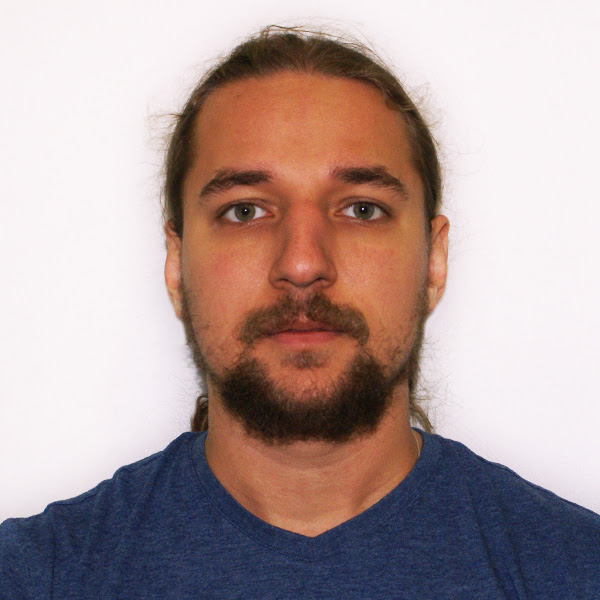
\includegraphics[width=\linewidth]{resources/photo.jpg}	%trimming relative to image size

%---------------------------------------------------------------------------------------
%	META SKILLS
%----------------------------------------------------------------------------------------
	\fcolorbox{white}{white}{\begin{minipage}[c][1.5cm][c]{1\mpwidth}
		\LARGE{\textbf{\textcolor{maincol}{Mike Lubinets}}} \\[2pt]
		\normalsize{ \textcolor{maincol} {Senior Rust Developer} }
\end{minipage}} \\

\icontext{CaretRight}{12}{Living in Berlin}{black}\\[6pt]
\icontext{CaretRight}{12}{Open to relocation}{black}\\[6pt]

\cvsection{Skills}

\cvskill{GNU/Linux} {8+ yrs.} {0.8} \\[-2pt]

\cvskill{Rust} {4+ yrs.} {0.9} \\[-2pt]

\cvskill{Research \& Development} {3+ yrs.} {0.64} \\[-2pt]

\cvskill{Distributed legder \newline technology} {3+ yrs.} {0.5} \\[-2pt]

\cvskill{Web development} {3+ yrs.} {0.4} \\[-2pt]

\cvskill{Embedded Systems} {1+ yrs.} {0.3} \\[-2pt]

\cvskill{English} {C1} {0.8} \\[-2pt]

\newpage
%---------------------------------------------------------------------------------------
%	EDUCATION
%----------------------------------------------------------------------------------------
\cvsection{Education}

\cvmetaevent
{2016 - 2018}
{Computer Science (B.Sc.)}
{Innopolis University}
{GPA: \textit{3.44} \newline Bachelor's thesis: \glqq Modular Language Server for SLang Programming Language\grqq.}

\cvmetaevent
{2014 - 2016}
{Computer Science (B.Sc.)}
{Saint Petersburg State University of Aerospace and Instrumentation}

%
\cvsection{Projects}
\cvlist{
	\item \hyperlink{https://github.com/mersinvald/aquamarine}{\textbf{aquamarine}}\\ Inline diagrams for rustdoc, used by Google
	\item \hyperlink{https://github.com/mersinvald/reed-solomon-rs}{\textbf{reed-solomon-rs}}\\ Reed-Solomon BCH implementation in Rust
	\item \hyperlink{https://github.com/mersinvald/batch_resolve}{\textbf{batch-resolver}} \\ Batch asynchronous DNS resolver
	\item \hyperlink{https://github.com/mersinvald/disciplinator}{\textbf{disciplinator}}\\ Hobby project to break sedentary lifestyle using FitBit API
	\item \hyperlink{https://crates.io/users/mersinvald}{\textbf{crates.io/users/mersinvald}}\\ Other small libraries and tools contributed to Rust ecosystem
}

\cvsection{Interests}

\icontext{CaretRight}{12}{Hiking}{black}\\[6pt]
\icontext{CaretRight}{12}{DIY}{black}\\[6pt]
\icontext{CaretRight}{12}{Programmable Keyboards}{black}\\[6pt]
\icontext{CaretRight}{12}{Cooking}{black}\\[6pt]
\icontext{CaretRight}{12}{Winter Sports}{black}\\[6pt]

\cvsection{Contact}

\icontext{MobilePhone}{16}{+49 176 27 95 28 13}{black}\\[6pt]
\iconemail{Envelope}{16}{me@mkl.dev}{me@mkl.dev}{black}\\[6pt]
\iconhref{Github}{16}{github.com/mersinvald}{https://www.github.com/mersinvald}{black}\\[6pt]
	
%\cvqrcode{0.3}

\end{leftcolumn}
\begin{rightcolumn}
%---------------------------------------------------------------------------------------
%	TITLE  HEADER
%----------------------------------------------------------------------------------------


%---------------------------------------------------------------------------------------
%	PROFILE
%----------------------------------------------------------------------------------------
\cvsection{About}
\vspace{4pt}

\cvtext{
    I am a Rust enthusiast who enjoys taking part in creation of new products 
    and making them reliable and loved. \\
    Currently I'm looking for on-site opportunities in Germany or relocation options in other countries,
    which would allow me to grow professionally while I'm preparing for my MSc. I'm looking forward to fulfill myself in a job that has engaging tasks,
    improves my current life quality and offers compelling benefits. \\
    If this profile fits you, you are very welcome to reach out.
}


%---------------------------------------------------------------------------------------
%	WORK EXPERIENCE
%----------------------------------------------------------------------------------------

\vspace{10pt}
\cvsection{Work experience}
\vspace{4pt}


\cvevent
{Oct/2019 - today}
	{Senior Rust Developer}
	{peaq GmbH}
    {
		My main occupation at peaq was the production of the peaq DLT platform and the related
		products. I have been working on the smart contracts execution runtime, blockchain storage, 
		and the implementation of the business requirements into the smart contracts running on the said platform. 
		\vfill\null
        Additionally, there was the management side of the job: I served as a representative of the
        peaq tech department in the meetings with potential clients and provided guidance and mentorship for the junior tech
		staff. 
		\vfill\null
		During my time at peaq, I have:
		\begin{itemize}
			\setlength\itemsep{-0.1em}
			\item successfully delivered the IoT and business logic parts of the technical PoC demo for the big partner in German automotive industry.
			\item designed and implemented the core layer of the blockchain-backed role based access control system, which later became the company's flagship product.
			\item lead the integration of the said RBAC system at the NTT datacenter, inpartnership with FATH Mechatronics.
			\item been a part of the great hard-working team, which didn't miss a single tight deadline (and there were many!)
		\end{itemize}
		\textit{Technical Stack}: Rust, C++, CLang Sanitizers, Exonum, RocksDB, GitLab CI, Docker
	}
	\vfill\null

\cvevent
{Jul/2018 - May/2019}
	{Rust Developer}
	{Ethereum Classic Labs\newline EVM/Compiler Team\newline Tooling Team}
	{
		I has been in charge of development and maintenance of the SputnikVM Ethereum Virtual Machine,
		as well as its integration into several Ethereum Clients, such as \textit{go-ethereum} and \textit{multi-geth}.
		\vfill\null
		Later, I switched to the tooling team, and worked on the Rust instruments around the OpenRPC protocol definition standard.
		\vfill\null
		During my time at ETCLabs, I have:
		\begin{itemize}
			\setlength\itemsep{-0.1em}
			\item released SputnikVM 0.11, that allowed integration of the VM into the cross-chain clients that support multiple Ethereum-based networks.
			\item streamlined the EVM testing framework used by SputnikVM, which allowed us to use whole Ethereum VM test suite.
			\item implemented support of Spurious Dragon, Byzantium and Constantinople sets of EIPs.
			\item maintained a number of other products implemented in Rust.
		\end{itemize}
		\textit{Technical Stack}: Rust, C, Go, JsonRPC, Ethereum, Jenkins CI, Docker, Vagrant
	}
	\vfill\null	
	\vfill\null
	
\cvevent
{Oct/2017 - Jul/2018}
	{Freelance Rust Developer}
	{Zamar AG}
	{
		As a freelance Rust developer I implemented a number of services for the client Airline Baggage processing system, 
		including IATA/BagMessage protocol implementation in Rust.
		\vfill\null
		Each module has been designed to be panic-free, highly reliable and performant.
		\vfill\null
		\textit{Technical Stack}: Async Rust, Tokio, SOAP, PostgreSQL
	}
	\vfill\null
	
\cvevent
    {Mar/2017 - Jul/2018}
	{Systems C Developer}
	{AnP Workcell\newline Systems Software Team}
	{
		Being an intern in the Systems Software team, I have ported parts of \textit{uclibc-ng}
		to the \textit{Elbrus e2k} processor architecture, established a continuous integration 
		infrastructure for running automation tests of the Linux Kernel and libc Elbrus builds,
		using Gitlab CI. The generated test reports have helped our team tremendously with keeping track of
		thousands of regressions.
		\vfill\null
		\textit{Technical Stack}: C, GDB, Valgring, GNU/Linux
	}
	\vfill\null

\cvevent
	{Nov/2015 - Jul/2016}
	{Trainee Embedded C++ Developer}
	{GK Scout\newline New Products R\&D Team}
	{
		On my first job, I got the experience intoductory to the embedded development with Cortex-M, 
		and to the product software development in general.
		\vfill\null
		I have had little personal responsibilities, but at the end of my employment I gained a short list of personal achievements: 
		\begin{itemize}
			\setlength\itemsep{-0.1em}
			\item implemented a NAND-flash driver with wear-levelling and Reed-Solomon BCH based error correction.
			\item improved speed and reliability of the proprietary networking protocol implementation which allowed transport of 3x bigger packets on the same MCU.
			\item unexpectedly became an only developer on a prototype firmware project and finished it before the scheduled release date.
		\end{itemize}
		\textit{Technical Stack}: Embedded C, C++, ARM Cortex-M, GDB, JTAG
	}
	\vfill\null

\end{rightcolumn}
\end{paracol}
%---------------------------------------------------------------------------------------
%	Recommendations
%----------------------------------------------------------------------------------------
\pagebreak
\cvsection{Recommendations}
\vspace{4pt}

\cvevent
	{August 2019, Senior Thesis Advisor}
	{Eugene Zouev}
	{Professor — Innopolis University}
	{
		It is my pleasure to write this letter of recommendation for Mikhail Lubinets, whom I have known for 3 years as a student of Innopolis University. I was a supervisor for Mikhail’s undergraduate research and taught several classes that he took as a part of his educational program.
		\vfill\null
		As a student, Mikhail always displayed a consistently high level in all of my courses and his grades are a good indicator of his abilities. However, it doesn’t end there, as a truly investigative person, Mikhail always went an extra mile to extend his knowledge and skills, when interested in some topic. Having observed Mikhail in several courses (“Introduction to Programming II” and “Functional Programming and Scala”), that involve collaboration with other students, I can tell that he makes a good team player: responsible and always ready to help.
		\vfill\null
		Mikhail has graduated from Innopolis with a BS thesis project “Architecture of Modular Language Server for the SLang programming language” under my supervising. During his undergraduate research, Mikhail demonstrated strong work ethic, professionalism, and high motivation. He is quite disciplined, organized person; he has never had any trouble with meeting deadlines for his assignments.
		\vfill\null
		On a personal level, Mikhail can be characterized as a very sympathetic and communicative person.
		To sum up, I strongly recommend Mikhail as a candidate for a research or work position without any reservations.
		\vfill\null
		Should you have any more questions feel free to contact me for further information.
	}
	\vfill\null

\cvevent
	{August 2019, Fellow Student}
	{Alena Iureva}
	{MSc in Data Engineering — Jacobs University Bremen}
	{
		Leading a student community is a busy and challenging thing to do, and I am happy I had Mike here nearby, with him taking care of study groups on courses he was best at, and helping out at admin stuff like planning and supplies.
		\vfill\null
		He is, as well, a true enthusiast and evangelist of Rust, who eventually got me to try the language and start contributing to open-source time to time, which led me to overall wider communication with international IT community.
		\vfill\null
		Mike has been leading by example, and a lot, being highly competitive and pushing us all to test our limits in abilities to accomplish better results, faster, showing example of impeccable confidence and I-can-do-it attitude. At the same time, he is always ready to help should someone be asking or seeking answers, taking his time to explain, review or give feedback.
		\vfill\null
		Overall, I see him as someone who really enjoys his work and wants to acquire as much expertise at it as possible, and I still keep hearing about projects he starts in his free time, or exciting new technologies he’s currently learning.
	}
	\vfill\null

\cvevent
	{March 2019, Direct Manager}
	{Darcy Reno}
	{Managing Director at ETCDEV Team}
	{
		Mike is a pleasure to work with - He has an excellent work ethic and is always looking for ways to make improvement in the product, the process and himself. I would gladly work with him in the future!
	}
	\vfill\null


% hofixes to create fake-space to ensure the whole height is used
\mbox{}
\vfill
\mbox{}
\vfill
\mbox{}
\vfill
\mbox{}
\vfill
\mbox{}
\vfill
\mbox{}
\vfill
\mbox{}


\end{document}